\chapter{Test Environment}
\label{cha:tests}

\newcommand{\gentestexec}{scafacos\_test}
\newcommand{\gentestdir}{tests/generic}

\section{Generic Test Program \texttt{\gentestexec}}

\noindent
The generic test program \texttt{\gentestexec} located in \texttt{\gentestdir} can be used to perform precision and performance tests with all solver methods in a common way.
The test case to be computed has to specified in form of an \emph{XML file}.
A single XML file can contain several particle configurations to be computed one after another using the same solver method.
The particle data (i.e., position and charge values as well as optional potential and field reference values) can either be read from the input file(s) (plain text or binary format) or generated \emph{online} using several internal particle data generators.
Furthermore, the particle system(s) to be computed can explicitly increased by duplicating the given input particles several times.
Additionally, the test program can write the result of the computations to a new XML output file.
This can be used to create potential and field reference values using one of the implemented solvers as reference method.

\subsubsection*{Usage:}

\begin{alltt}
  ./\gentestexec [OPTIONS] METHOD FILE
\end{alltt}

\noindent
The test program has to be executed in parallel using MPI (e.g. with \texttt{mpiexec -n NUMPROCS ./\gentestexec ...}).
\texttt{METHOD} specifies the solver method to be used and can be any method name supported by the FCS init function \texttt{fcs\_init} (see \ref{sec:init_step}).
Additionally, the method name can also be \texttt{none} to pass the test case through the test program (including parsing, particle data generation, duplication, and output), but without executing a solver.
\texttt{FILE} specifies the XML file describing the test case to be computed.
If the zlib compression library was available during building the library, then the XML files can also be compressed.
The command line arguments are only read on the master process.

\subsubsection*{Options:}

\noindent
The given command line arguments override conflicting settings that may already exist within the XML file that specifies the test case.

\begin{tabular}{lp{0.8\textwidth}}

\texttt{-o OUTFILE} &
Write the given test case including the computed results to a new XML file \texttt{OUTFILE}.
\\
\texttt{-b} &
Write the particle data in a machine-dependent binary format to a separate file (basename of \texttt{OUTFILE} with 'bin' suffix.
This is only useful together with \texttt{-o} option.
\\
\texttt{-d DUP} &
Duplicate a given periodic particle system in each \emph{periodic} dimension.
\texttt{DUP} can be a single value X or three values XxYxZ (i.e., one separate value for each dimension).
The default value of \texttt{DUP} = 1 is equivalent to no duplication.
\\
\texttt{-m MODE} &
Specify how the input particle data is distributed among parallel processes before the solver is executed.
Mode can be one of the following:
\begin{compactitem}
  \item \texttt{atomistic}: Equal distribution without any further assumptions (this is the \emph{default}).
  \item \texttt{all\_on\_master}: All particles are on the master process.
  \item \texttt{random}: Equal distribution after a random redistribution.
  \item \texttt{domain}: Redistribution depending on the particle positions.
This represents a regular domain decomposition with respect to a Cartesian grid of MPI processes.
The process grid is created by MPI and supplied to the solver in form of a Cartesian communicator.
\end{compactitem}
\\
\texttt{-c CONF} & Set additional method configuration parameters. \texttt{CONF} is given to FCS function \texttt{fcs\_parser} (see \ref{}).
\\
\texttt{-i ITER} & Perform \texttt{ITER} number of runs with each configuration.
\\
\texttt{-r RES} &
Compute results only for \texttt{RES} of the given particles, where \texttt{RES} can be an absolute integer number of particles (i.e., without '.') or a fractional number (i.e., with '.') relative to the given particles.
The default value \texttt{RES}=1.0 is equivalent to all particles.
If the direct solver is used, then all other particles (i.e., the particles for which no results are computed) are used as additional input particles for the computations.
\end{tabular}


\subsection*{Text case XML file format}

\noindent
The XML file contains all necessary information to describe the particle configurations to be computed.
The master process reads the whole XML file at once and stores the information of all particle configurations in its local memory.
Plain text particle data contained in the XML file is also stored at once on the master process.
Input of binary particle data as well as any generation or duplication of particle data is performed by all processes in parallel just before the corresponding particle configuration is prepared for the computations.
The root element of the test case XML file is called \texttt{scafacos\_test}.

\begin{center}
\small
\begin{tabular}{|p{3cm}|p{1.5cm}|p{8.5cm}|}
  \hline
  \textit{Element}           & \multicolumn{2}{p{10cm}|}{\texttt{<scafacos\_test>}\dots\texttt{</scafacos\_test>}} \\ \hline
  \textit{description}       & \multicolumn{2}{p{10cm}|}{Root element of the test case XML file} \\ \hline
  \textit{Child-elements}    & \multicolumn{2}{p{10cm}|}{\texttt{<configuration>*}} \\ \hline
  \hline
  \textbf{Attributes}        & \textbf{Type} & \textbf{Description} \\ \hline
  \texttt{name}              & string & Name of the test case. \\ \hline
  \texttt{description}       & string & One-line description of the test case. \\ \hline
  \texttt{reference\_method} & string & Name of the method used to compute the reference potential and field values. \\ \hline
  \texttt{error\_potential}  & string & Estimated maximal error of the reference potential values. \\ \hline
  \texttt{error\_field}      & string & Estimated maximal error of the reference field values. \\ \hline
\end{tabular}
\end{center}

\noindent
Each test case XML file can contain several particle configurations that should be computed one after another using the same solver method.
The XML element specifying a particle configuration is call \texttt{configuration}.
Child-elements are used to add particles in form of plain text or binary particle data as well as through the particle generators or explicit duplication of given particles.
There can be an arbitrary number of \texttt{particle}, \texttt{binary}, and \texttt{generate} elements.
There can be only one \texttt{duplicate} element that specifies the duplication for \emph{all} given particles.

\begin{center}
\small
\begin{tabular}{|p{3cm}|p{1.5cm}|p{8.5cm}|}
  \hline
  \textit{Element}        & \multicolumn{2}{p{10cm}|}{\texttt{<configuration>}\dots\texttt{</configuration>}} \\ \hline
  \textit{Description}    & \multicolumn{2}{p{10cm}|}{Particle configuration to be computed.} \\ \hline
  \textit{Child-elements} & \multicolumn{2}{p{10cm}|}{\texttt{<particle>*}, \texttt{<binary>*}, \texttt{<generate>*}, \texttt{<duplicate>}} \\ \hline
  \hline
  \textbf{Attributes}     & \textbf{Type} & \textbf{Description} \\ \hline
  \texttt{offset}         & float[3] & Origin of the system box. \\ \hline
  \texttt{box\_a}         & float[3] & First base vector of the system box. \\ \hline
  \texttt{box\_b}         & float[3] & Second base vector of the system box. \\ \hline
  \texttt{box\_c}         & float[3] & Third base vector of the system box. \\ \hline
  \texttt{periodicity}    & bool[3]  & Periodicity of the system. \\ \hline
  \texttt{epsilon}        & float or \newline 'metallic' & Value of the dielectric permittivity of the system boundary. Use 'metallic' for infinite permittivity, i.e. metallic boundary conditions. \\ \hline
  \texttt{decomposition}  & string & Input particle distribution: 'atomistic', 'all\_on\_master', 'random', or 'domain'. See the description of the \texttt{-m} option of the test program for further information about the difference input distributions. \\ \hline
\end{tabular}
\end{center}

\subsection*{Plain text and binary particle data input}

\noindent
A single particle can be specified as plain text within the XML file using the \texttt{particle} element.
The attributes of this element are used to specify the position, charge, reference potential, and reference field values.
There can be an arbitrary number of these \texttt{particle} elements.

\begin{center}
\small
\begin{tabular}{|p{3cm}|p{1.5cm}|p{8.5cm}|}
  \hline
  \textit{Element}        & \multicolumn{2}{p{10cm}|}{\texttt{<particle>}\dots\texttt{</particle>}} \\ \hline
  \textit{Description}    & \multicolumn{2}{p{10cm}|}{Data of a single particle.} \\ \hline
  \textit{Child-elements} \\ \hline
  \hline
  \textbf{Attributes}     & \textbf{Type} & \textbf{Description} \\ \hline
  \texttt{position}       & float[3]      & Position of the particle. \\ \hline
  \texttt{q}              & float         & Charge of the particle. \\ \hline
  \texttt{potential}      & float         & Reference potential at the position of the particle. \\ \hline
  \texttt{field}          & float[3]      & Reference field at the position of the particle. \\ \hline
\end{tabular}
\end{center}

\noindent
Binary particle data input from a separate file can be specified with the \texttt{binary} element.
The attributes of this element are used to specify the filename, offset, and total number of particles to read.
Position, charge, reference potential, and reference field values are only read if the corresponding child-elements are present within the \texttt{binary} element.
The binary particle data is read by all processes in parallel using MPI I/O.

\begin{center}
\small
\begin{tabular}{|p{3cm}|p{1.5cm}|p{8.5cm}|}
  \hline
  \textit{Element}        & \multicolumn{2}{p{10cm}|}{\texttt{<binary>}\dots\texttt{</binary>}} \\ \hline
  \textit{Description}    & \multicolumn{2}{p{10cm}|}{Binary particle data input from a separate file.} \\ \hline
  \textit{Child-elements} & \multicolumn{2}{p{10cm}|}{\texttt{<positions>}, \texttt{<charges>}, \texttt{<potentials>}, \texttt{<field>}} \\ \hline
  \hline
  \textbf{Attributes}     & \textbf{Type} & \textbf{Description} \\ \hline
  \texttt{file}           & string        & Filename of the input file. \\ \hline
  \texttt{offset}         & int           & Offset in bytes within the input file. \\ \hline
  \texttt{ntotal}         & int           & Total number of particles to read. \\ \hline
\end{tabular}
\end{center}

\subsection*{Particle data duplication}

\noindent
The \texttt{duplicate} element is used to specify how often the given particles should be duplicated in each dimension.
The particle positions can optionally be scaled back to the original size of the system box.

\begin{center}
\small
\begin{tabular}{|p{3cm}|p{1.5cm}|p{8.5cm}|}
  \hline
  \textit{Element}        & \multicolumn{2}{p{10cm}|}{\texttt{<duplicate>}\dots\texttt{</duplicate>}} \\ \hline
  \textit{Description}    & \multicolumn{2}{p{10cm}|}{Explicit duplication of the given input particles (additionally to the duplication specified on the command line).} \\ \hline
  \textit{Child-elements} & \multicolumn{2}{p{10cm}|}{\texttt{<particle>*}, \texttt{<binary>*}, \texttt{<generate>*}} \\ \hline
  \hline
  \textbf{Attributes}     & \textbf{Type} & \textbf{Description} \\ \hline
  \texttt{times}          & int[3]        & Number of times the given input particles should be duplicated in each dimension. Value '1 1 1' corresponds to no duplication. \\ \hline
  \texttt{rescale}        & bool          & Whether the particle positions should be scaled back to the original system size after the duplication. \\ \hline
\end{tabular}
\end{center}

\subsection*{Particle data generators}

\noindent
The test program contains several generators that can be used to create particle data for arbitrary large particle configurations.
The \texttt{generate} element can be used to specify the generation of a set of particles.
Particle data generators are executed by all processes in parallel such that each process creates only its locally required particles.
The generation of position, charge, reference potential, and reference field values are be specified independently from each other.

\begin{center}
\small
\begin{tabular}{|p{3cm}|p{1.5cm}|p{8.5cm}|}
  \hline
  \textit{Element}        & \multicolumn{2}{p{10cm}|}{\texttt{<generate>} \dots \texttt{</generate>}} \\ \hline
  \textit{Description}    & \multicolumn{2}{p{10cm}|}{Generator for particle data} \\ \hline
  \textit{Child-elements} & \multicolumn{2}{p{10cm}|}{\texttt{<positions>}, \texttt{<charges>}, \texttt{<potentials>}, \texttt{<field>}} \\ \hline
  \hline
  \textbf{Attributes}     & \textbf{Type} & \textbf{Description} \\ \hline
  \texttt{nlocal}         & int           & Local number of particles to generate on each process. \\ \hline
  \texttt{ntotal}         & int or int[3] & Total number of particles to generate. Three values can be used to specify the number of particles to generate for a grid of particles. \\ \hline
\end{tabular}
\end{center}

\noindent
The generation of particle positions consists of the type of input values to use and of a shape in which these input values are transformed to.
Both type and shape can be specified as attributes of the \texttt{positions} element.

\begin{center}
\small
\begin{tabular}{|p{3cm}|p{1.5cm}|p{8.5cm}|}
  \hline
  \textit{Element}        & \multicolumn{2}{p{10cm}|}{\texttt{<positions>} \dots \texttt{</positions>}} \\ \hline
  \textit{Description}    & \multicolumn{2}{p{10cm}|}{Parameters for generating particle positions.} \\ \hline
  \hline
  \textbf{Attributes}     & \textbf{Type} & \textbf{Description} \\ \hline
  \texttt{type}           & string        & Use 'random', 'hammersley', or 'halton' to create corresponding sequences of input values. These values are transformed into the specified shape. Use 'grid' to create equally spaced particles. In this case, the three values within the \texttt{ntotal} attribute of the enclosing \texttt{generate} element are used to specify the number of particles in each dimension of the grid.
 \\ \hline
  \texttt{shape}          & string        & Use the generate sequences of input values to create a particle distribution shaped like a 'box', 'ball', or the surface of a 'sphere'. Furthermore, two way of creating plummer distributions are available ('plummer' and 'plummer\_ball'). All distributions are scaled to fit into the given system box. \\ \hline
\end{tabular}
\end{center}

\noindent
Particle charges, reference potential, and reference field values can either be set to a single constant value or a list of alternating values.

\begin{center}
\small
\begin{tabular}{|p{3cm}|p{1.5cm}|p{8.5cm}|}
  \hline
  \textit{Element}        & \multicolumn{2}{p{10cm}|}{\texttt{<charges>}\dots\texttt{</charges>}, \newline \texttt{<potentials>}\dots\texttt{</potentials>}, \newline \texttt{<field>}\dots\texttt{</field>}} \\ \hline
  \textit{Description}    & \multicolumn{2}{p{10cm}|}{Parameters for generating particle charges, reference potentials, and reference field values.} \\ \hline
  \textit{child-elements} & none \\ \hline
  \hline
  \textbf{Attributes}     & \textbf{Type} & \textbf{Description} \\ \hline
  \texttt{type}           & string        & Use 'const' or 'alternate' to set the particle data to a single constant value or to a list of alternating values, respectively. \\ \hline
  \texttt{value}          & float[*]      & Constant or alternating value(s) to use. \\ \hline
\end{tabular}
\end{center}


\section{Numerical Results}\label{sec:numerik}
%
\section{Generation of Simulation Data}

We consider Hammersley- and Halton sequences \cite{wong97a}.  These
sequences provide pseudo random numbers such that the distance between
two particles does not become too small.  We use the program
\textit{HAMMERSLEY} \cite{hammersley} from John Burkardt to generate
these sequences.

These sequences are defined as follows: Let $p$ prime. Each number
$k\in \mathbb N$ can be uniquely represented as
\[
k = a_0 + a_1 p + a_2 p^2 + \ldots + a_r p^r,
\]
with $r\in\mathbb N$ and $a_i \in \left\{0,\hdots,p-1 \right\}$,
$i=0,\hdots,r$. The function $\Phi_p(k)$ is given by
\[
\Phi_p(k) = \dfrac{a_0}{p} + \dfrac{a_1}{p^2} + \dfrac{a_2}{p^3} +
\ldots + \dfrac{a_r}{p^{r+1}}.
\]

\paragraph{Hammersley Sequences}
Let the dimension $d$ and prime numbers $p_1, p_2, \ldots, p_{d-1}$
with $p_1 < p_2 < \ldots < p_{d-1}$ be given. Furthermore let $N$ the
number of particles.  The $k$-th $d$-dimensional particle of the
Hammersley distribution is given by
\[
  \left( \dfrac{k}{N}, \Phi_{p_1}(k), \Phi_{p_2}(k), \ldots, \Phi_{p_{d-1}}(k) \right), \textbf{   } k=0,\ldots,N-1.
\]

\paragraph{Halton Sequences}
Let in addition a prime number $p_d$ with $p_{d-1} < p_d$ given.  The
$k$-th $d$-dimensional particle of the Halton distribution is given by
\[
  \left( \Phi_{p_1}(k), \Phi_{p_2}(k), \ldots, \Phi_{p_d}(k) \right), \textbf{   } k=0,\ldots,N-1.
\]
Since each component of the $k$-th particle is independent of $N$, one
can produce additional particles.

\section{Error}

In order to demonstrate the efficiency of our methods with a more
simple discrete sum we start with the calculation of the potential
$\varphi$ caused by $N$ charged particles with charges $q_\ell$ given
by
\[
  \varphi(\mathbf r_j) =
  \sum_{\overset{\ell=1}{j\not=\ell}}^{N} \frac{q_\ell}{\|\mathbf r_j-\mathbf
  r_{\ell}\|}\, , \qquad (\mathbf r_j\in {\mathbb R}^3). 
\]
the force
\[
  \boldsymbol{F}\left(\boldsymbol{r}_j\right) :=
  \left(\rule{0pt}{2.0ex}\, F_0\left(\boldsymbol{r}_j\right),F_1\left(\boldsymbol{r}_j\right), F_2\left(\boldsymbol{r}_j\right)\, \right)^\top =
  - q_j \, \nabla \varphi\left(\boldsymbol{r}_j\right)
\]
the energy
\[
  E := \frac{1}{2} \sum\limits_{j=1}^{N} q_j \,
  \varphi\left(\boldsymbol{r}_j\right) = 
  \frac{1}{2} \sum\limits_{j=1}^{N} q_j \, 
  \underset{\ell\neq j}{\sum\limits_{\ell=1}^{N}} 
  \frac{q_j}{\left\Vert \boldsymbol{r}_j - 
  \boldsymbol{r}_\ell \right\Vert_2}
\]
and the virial
\[
 ???
\]
We investigate the numerical error
\[
  \mathcal{E}^{\varphi}_{2}(\mbox{a,b}) = \left(\displaystyle \sum_{k=1}^{N} |\varphi_{\mbox{\tiny a}}
  (\mathbf r_k)-\varphi_{\mbox{\tiny b}}(\mathbf r_k)|^2\right)^{1/2}
  \left(\displaystyle\sum_{k=1}^{N}|\varphi_{\mbox{\tiny a}}(\mathbf r_k)|^2\right)^{-1/2}\, ,
\]
\[
  \mathcal{E}_{2}^{\boldsymbol F}(\mbox{a,b})
  = \left(\displaystyle
    \sum_{k=1}^{N} \|\mathbf F_{\mbox{\tiny a}}(\mathbf r_k)-\mathbf F_{\mbox{\tiny b}}(\mathbf r_k)\|^2_2\right)^{1/2}
    \left(\displaystyle\sum_{k=1}^{N}\|\mathbf F_{\mbox{\tiny a}}(\mathbf r_k) \|^2_2\right)^{-1/2}\;
\]
and
\[
  \mathcal{E}_{2}^{E}(\mathrm{a},\mathrm{b})
  = \frac{|E_{\mathrm{a}}-E_{\mathrm{b}}|}{|E_{\mathrm{a}}|}
\]
where $\mathrm{a}$ and $\mathrm{b}$ represent the different techniques
for the computation.  Furthermore we investigate the sum
$\boldsymbol{F}_\mathrm{S}(\mathrm{a}) = \sum_{j=1}^{N}
\boldsymbol{F}\left(\boldsymbol{r}_j\right)$, which should be zero and
compute $F_\mathrm{S}(a) := \left\Vert
  \boldsymbol{F}_\mathrm{S}(\mathrm{a}) \right\Vert_\infty$.

\section{Distributions and Results}
\label{sec:VertErg}
\subsection{Distribution \texttt{hammersley\_ball}}
We consider Hammersley sequences in the cube $\left[0 , 1 \right]^3$
generated by $p_1 = 2$, $p_2 = 3$, and, finally, projected in the ball
\[
(x-0.5)^2 + (y-0.5)^2 + (z-0.5)^2 \leq (0.5)^2.
\]
We choose the charges $q_\ell \in \left\lbrace -1 ; 1\right\rbrace$
random such that
\[
  \sum\limits_{\ell=1}^{N} q_\ell \in \left\lbrace -1 ; 0; 1\right\rbrace.
\]

\begin{figure}[ht]
  \centering
  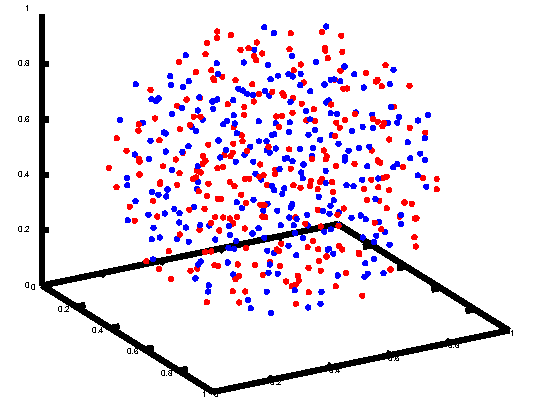
\includegraphics[width=0.5\textwidth]{figures/hball_500}
  \caption{Distribution \texttt{hammersley\_{}ball} with 500 randomly charged particles.}
\end{figure}

We choose the following parameter for our tests.

\begin{table}[p]
  \begin{footnotesize}
    \begin{center}
      \begin{tabular}{|r||c|c|c|c||c|c|c|c|}
        \hline \rule{0cm}{2.5ex}
        & \multicolumn{4}{c|}{FMM} & \multicolumn{4}{c|}{P2NFFT} \\
        \hline \rule{0cm}{2.5ex}
        N & ??? & ??? & ??? & ??? & $n$ & $m$ & $p$ & $\varepsilon_{I} = \varepsilon_{B}$ \\
        \hline
        500      & ??? & ??? & ??? & ??? & 32,32,32 & 2 & 5 & 3.5/32 \\
        5\,000   & ??? & ??? & ??? & ??? & 32,32,32 & 2 & 5 & 3.5/32 \\
        50\,000  & ??? & ??? & ??? & ??? & 64,64,64 & 2 & 5 & 3.5/64 \\
        500\,000 & ??? & ??? & ??? & ??? & 128,128,128 & 2 & 5 & 3.5/128 \\
        \hline
      \end{tabular}
    \end{center}
  \end{footnotesize}
  \caption{Parameters for the distribution \texttt{hammersley\_{}ball}}
\end{table}


\begin{table}[p]
  \centering
  \begin{tabular}{|r||r|r|r||c|c|}
    \hline
    $N$ & $t_\textrm{direct}$ & $t_\textrm{FMM}$ & $t_\textrm{P2NFFT}$ &
    \rule{0cm}{3ex}
    ${\cal E}^{\varphi}_2\left(\textrm{direct},\textrm{FMM}\right)$ &
    ${\cal E}^{\varphi}_2\left(\textrm{direct},\textrm{P2NFFT}\right)$ \\
    \hline
    500 & ??? & ??? & ??? & ??? & ??? \\
    5\,000 & ??? & ??? & ??? & ??? & ??? \\
    50\,000 & ??? & ??? & ??? & ??? & ??? \\
    500\,000& * & ??? & ??? & * & * \\
    \hline
  \end{tabular}
  \caption{Time and Error for 32 processes}
\end{table}

\begin{table}[p]
  \centering
  \begin{tabular}{|r||r|r||c|c|}
    \hline
    $P$ & $t_\textrm{FMM}$ & $t_\textrm{P2NFFT}$ &
    \rule{0cm}{3ex}
    ${\cal E}^{\varphi}_2\left(\textrm{ref},\textrm{FMM}\right)$ &
    ${\cal E}^{\varphi}_2\left(\textrm{ref},\textrm{P2NFFT}\right)$ \\
    \hline
    32   & ??? & ??? & ??? & ??? \\
    128  & ??? & ??? & ??? & ??? \\
    512  & ??? & ??? & ??? & ??? \\
    2048 & ??? & ??? & ??? & ??? \\
    8192 & ??? & ??? & ??? & ??? \\
    \hline
  \end{tabular}
  \caption{Strong scaling for $N=1\,000\,000$ particles and error bound ${\cal E}^{\varphi}_2 \le 10^{-4}$}
\end{table}

\begin{table}[p]
  \centering
  \begin{tabular}{|r||r|r||c|c|}
    \hline
    $P$ & $t_\textrm{FMM}$ & $t_\textrm{P2NFFT}$ &
    \rule{0cm}{3ex}
    ${\cal E}^{\varphi}_2\left(\textrm{ref},\textrm{FMM}\right)$ &
    ${\cal E}^{\varphi}_2\left(\textrm{ref},\textrm{P2NFFT}\right)$ \\
    \hline
    32   & ??? & ??? & ??? & ??? \\
    128  & ??? & ??? & ??? & ??? \\
    512  & ??? & ??? & ??? & ??? \\
    2048 & ??? & ??? & ??? & ??? \\
    8192 & ??? & ??? & ??? & ??? \\
    \hline
  \end{tabular}
  \caption{Weak scaling for $N=1\,000\,000$ particles per process and error bound ${\cal E}^{\varphi}_2 \le 10^{-4}$}
\end{table}

\subsection{Distribution \texttt{hammersley\_{}ball\_{}neg\_{}charge}}

As numerical test we used a ball uniformly filled with charged particles. The
total charge of the ball has been kept with $Q=-$1~nC. Thus the particles are assumed to
posses the charge $q_\ell=q=-1/N$~nC $(\ell=1,\dots,N)$, where $N$ denotes the number of
particles in the ball. These particles are also regarded as macro-particles representing
the distribution of all particles (for instance electrons) in a bunch. 

\begin{figure}[ht]
  \centering
  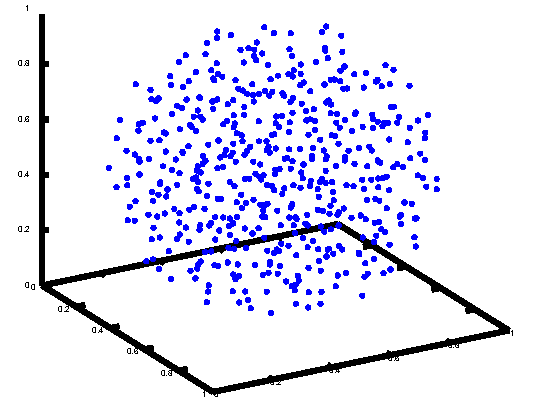
\includegraphics[width=0.5\textwidth]{figures/hballneg_500}
  \caption{Distribution \texttt{hammersley\_{}ball} with 500 negative charged particles.}
\end{figure}

Since a ball uniformly filled with an increasing number of particles
of equal charge gets more and more close to a ball with charge
$Q=\sum_{\ell=1}^N q_\ell$, we compare the results of the summation to
the analytically known potential of a homogeneously charged ball given
by (normalized by the factor $4\pi\varepsilon_0$)
% \[
%   \varphi_{\mbox {\tiny asym}}(\mathbf r_j)
%   = \frac{Q}{4\pi\varepsilon_0} \left(
%     \frac{3}{2}-\frac{\|\mathbf r_j\|}{2 R^2}\right)\, ,\qquad \|\mathbf r_j\|\leq R,
% \]
%% omit scaling with 1/(4*pi*eps0)
\[
  \varphi_{\mbox {\tiny asym}}(\mathbf r_j)
  = \frac{Q}{4\pi\varepsilon_0} \left(
    \frac{3}{2}-\frac{\|\mathbf r_j\|}{2 R^2}\right)\, ,\qquad \|\mathbf r_j\|\leq R,
\]
where $R$ denotes the radius of the ball.\par

\begin{table}[htb]
  \centering
  \begin{tabular}{|c||c|c|c|c|c|c|}
    \hline \rule{0mm}{5mm}
    $N$ & $t_{\mbox{\tiny slow}}$  &   $t_{\mbox{\tiny fast}}$
    &$\mathcal{E}_{2}^{\varphi}(\mbox{asym,slow})$
    &$\mathcal{E}_{2}^{\varphi}(\mbox{asym,P2NFFT})$
    &$\mathcal{E}_{2}^{\varphi}(\mbox{slow,P2NFFT})$  \\ \hline
    10\,000     & ??? & ??? & ??? & ??? &  ??? \\ \hline
    50\,000     & ??? & ??? & ??? & ??? &  ??? \\ \hline
    100\,000    & ??? & ??? & ??? & ??? &  ??? \\ \hline
    250\,000    & *   & ??? & *   & ??? &  *   \\ \hline
    500\,000    & *   & ??? & *   & ??? &  *   \\ \hline
    1\,000\,000 & *   & ??? & *   & ??? &  *   \\ \hline
  \end{tabular}
  \caption{Computational time and the error $\mathcal{E}_{2}$ for the potential $\varphi$, *estimated.\label{e2_potential}}
\end{table}
%
The numerical experiments documented in Table~\ref{e2_potential} show
that we obtain with our fast algorithm the same errors as with the
straightforward (slow) summation but with an numerical effort of only
$\mathcal{O}(N\log N)$. Hereby the parameters of the P2NFFT are chosen
such that the approximation error is less than the simulation error.
Finally, we test the algorithm for the computation of the
electrostatic field.  It is well known that the field of a
homogeneously charged ball is given by (normalized by the factor
$4\pi\varepsilon_0$)
% \[
% \mathbf E_{\mbox {\tiny asym}}(\mathbf r_j)
% =\frac{Q}{4\pi\varepsilon_0} \left( \frac{\mathbf r_j}{R^3}\right)\,
% ,\qquad \|\mathbf r_j\|\leq R.
% \]
%% omit scaling with 1/(4*pi*eps0)
\[
  \mathbf E_{\mbox {\tiny asym}}(\mathbf r_j)
  = Q \left( \frac{\mathbf r_j}{R^3}\right)\,,\qquad \|\mathbf r_j\|\leq R.
\]

% Table~\ref{e2_efield} represents the results of the related numerical simulations.
% Figure~\ref{nfft_times} compares the performance of P2NFFT to the direct slow summation.
% It shows that P2NFFT scales with $\mathcal{O}(N\log N)$.
% The numerical errors are acceptable (see Table~\ref{e2_potential}).
% Hence this new summation technique enables the computation of
% fully 3D particle-particle interactions in real life applications.


%%% Local Variables: 
%%% mode: latex
%%% TeX-master: ug.tex
%%% End: 
